\begin{frame}[plain]
  \begin{center}
    \vspace{2em}
    {\LARGE\textbf{Vision-Language Models}}

    \vspace{2.5em}
    {\scriptsize Parts of this section adapted from D. Kiela, ``Multimodal Deep Learning (with an NLP focus)'',\\
    guest lecture, Stanford CS224n, Winter 2023.}
  \end{center}
\end{frame}

\begin{frame}{The Vision-Language Task Space}
  \begin{columns}[T,onlytextwidth]
    \column{0.54\textwidth}
      \begin{itemize}
        \item[{\color{red}\textbullet}] \textbf{Visual question answering:} free-form questions about an
          image (VQA, ICCV 2015). VQAv2 (CVPR 2017) pairs every question with two images that yield two
          different answers, so language priors alone cannot score well.
        \item[{\color{red}\textbullet}] \textbf{Captioning:} describe the image (COCO Captions: five
          human captions per image, CIDEr and BLEU scoring).
        \item[{\color{red}\textbullet}] \textbf{Referring expressions:} localize ``the man in the red
          hat'' (RefCOCO family, 2016).
        \item[{\color{red}\textbullet}] \textbf{Reading text in images:} TextVQA (CVPR 2019).
        \item[{\color{red}\textbullet}] \textbf{Documents and charts:} DocVQA (WACV 2021), ChartQA (ACL
          Findings 2022).
      \end{itemize}
    \column{0.42\textwidth}
      \begin{figure}
        \centering
        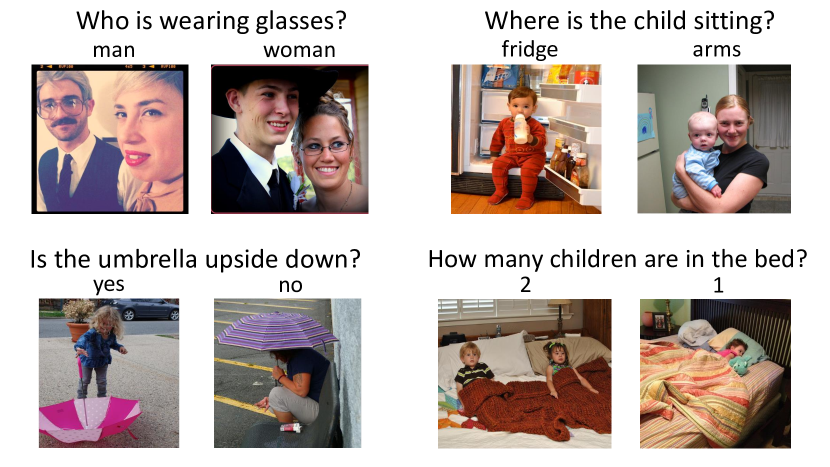
\includegraphics[width=\linewidth, height=0.56\textheight, keepaspectratio]{images/multimodal-nlp/multimodal_vqav2_complementary_pairs.png}
        \caption*{\scriptsize VQAv2's complementary pairs: same question, two images, two answers.
        Source: Goyal et al., ``Making the V in VQA Matter'', CVPR 2017,
        \href{https://arxiv.org/abs/1612.00837}{arXiv:1612.00837}, Figure~1.}
      \end{figure}
  \end{columns}
  \vspace{0.2em}
  {\scriptsize Multimodal LLMs are still evaluated on descendants of all five tasks.}
\end{frame}

\begin{frame}{CLIP in One Slide}
  \begin{itemize}
    \item[{\color{red}\textbullet}] \textbf{Contrastive Language-Image Pretraining} (Radford et al., ICML 2021): a dual
      encoder trained on 400M web (image, text) pairs so that each image ranks its own caption above
      the other captions in the batch, and each caption ranks its own image.
    \item[{\color{red}\textbullet}] \textbf{What it buys:} zero-shot classification from text prompts, image-text
      retrieval, and robustness to sketches, renditions and adversarial photographs that break
      supervised ImageNet models.
    \item[{\color{red}\textbullet}] \textbf{What it cannot do:} it only \emph{scores} image-text pairs. There is no
      decoder, so it cannot describe an image, answer a question, or hold a conversation.
    \item[{\color{red}\textbullet}] \textbf{Why it still matters:} contrastively pretrained encoders became the eyes
      of nearly every multimodal LLM that followed.
  \end{itemize}
  \vspace{0.4em}
  {\scriptsize Radford et al., ``Learning Transferable Visual Models From Natural Language Supervision'',
  ICML 2021, \href{https://arxiv.org/abs/2103.00020}{arXiv:2103.00020}.}
\end{frame}

\begin{frame}{The Contrastive Objective, Formally}
  For a batch $\mathcal{B}$ of $\ell_2$-normalized image embeddings $x_i$ and text embeddings $y_i$,
  CLIP minimizes a symmetric cross-entropy over temperature-scaled cosine similarities:
  \begin{equation*}
    \mathcal{L}_{\mathrm{softmax}} \;=\; -\frac{1}{2|\mathcal{B}|} \sum_{i=1}^{|\mathcal{B}|} \left(
      \log \frac{e^{t\, x_i \cdot y_i}}{\sum_{j} e^{t\, x_i \cdot y_j}}
      \;+\; \log \frac{e^{t\, x_i \cdot y_i}}{\sum_{j} e^{t\, x_j \cdot y_i}} \right)
  \end{equation*}
  The temperature $t$ is \emph{learned}, and both terms need the full batch similarity matrix.
  SigLIP replaces this with an independent binary decision per pair:
  \begin{equation*}
    \mathcal{L}_{\mathrm{sigmoid}} \;=\; -\frac{1}{|\mathcal{B}|} \sum_{i=1}^{|\mathcal{B}|} \sum_{j=1}^{|\mathcal{B}|}
      \log \frac{1}{1 + e^{\,z_{ij}\,(-t\, x_i \cdot y_j + b)}},
    \qquad z_{ij} = \begin{cases} \phantom{-}1 & i = j \\ -1 & i \neq j \end{cases}
  \end{equation*}
  with a learned bias $b$ offsetting the imbalance of negative pairs. Sigmoid training wins clearly
  below batch size 16k; both losses saturate around 32k.
  \vspace{0.2em}

  {\scriptsize Notation follows Zhai et al., ICCV 2023, \href{https://arxiv.org/abs/2303.15343}{arXiv:2303.15343},
  Secs.~3.1--3.2 (their formalization of the CLIP loss).}
\end{frame}

\begin{frame}{Vision Encoders After CLIP: SigLIP and SigLIP 2}
  \begin{itemize}
    \item[{\color{red}\textbullet}] \textbf{SigLIP} (Zhai et al., ICCV 2023) replaces CLIP's softmax contrastive loss
      with a pairwise \textbf{sigmoid} loss: every image-text pair becomes an independent binary
      decision, so the loss needs no global view of all pairings in the batch.
    \item[{\color{red}\textbullet}] \textbf{SigLIP 2} (Feb 2025) folds captioning-based pretraining, self-distillation,
      masked prediction and online data curation into one multilingual recipe, with much stronger
      localization and dense features.
    \item[{\color{red}\textbullet}] Its \textbf{NaFlex} variants support several resolutions and preserve the input's
      native aspect ratio; checkpoints range from ViT-B (86M) to g (1B).
    \item[{\color{red}\textbullet}] These encoders, more than CLIP itself, are what current open multimodal models
      plug in: LLaVA-OneVision and Janus-Pro use SigLIP, BAGEL uses SigLIP 2.
  \end{itemize}
  \vspace{0.4em}
  {\scriptsize Zhai et al., \href{https://arxiv.org/abs/2303.15343}{arXiv:2303.15343};
  Tschannen et al., \href{https://arxiv.org/abs/2502.14786}{arXiv:2502.14786}.}
\end{frame}

\begin{frame}{The Visual BERT Era (2019--2022)}
  Before decoder LLMs, vision-language pretraining meant BERT-style encoders over text and image features:
  \begin{itemize}
    \item[{\color{red}\textbullet}] \textbf{VisualBERT} (2019): one Transformer stack attends over text tokens and
      object-detector regions together (early fusion); masked language modelling \emph{with the image}.
    \item[{\color{red}\textbullet}] \textbf{ViLBERT} (NeurIPS 2019) and \textbf{LXMERT} (EMNLP 2019): two streams, one
      per modality, exchanging information through co-attention layers.
    \item[{\color{red}\textbullet}] \textbf{Pixel-BERT} (2020): drops the object detector; a CNN feeds pixel-level
      features straight to the Transformer.
    \item[{\color{red}\textbullet}] \textbf{FLAVA} (CVPR 2022): three towers (vision, language, multimodal) trained
      with masked and contrastive objectives on public data; one model for unimodal and multimodal tasks.
    \item[{\color{red}\textbullet}] \textbf{Why they faded:} they classify, score and retrieve over fixed label sets,
      each downstream task needs its own fine-tuned head, and none of them generates language.
  \end{itemize}
\end{frame}

\begin{frame}{From Dual Encoders to Multimodal LLMs}
  \begin{itemize}
    \item[{\color{red}\textbullet}] \textbf{Nomenclature.} An \textbf{LLM} is language-only. A
      \textbf{VLM} (vision-language model) adds a vision encoder so the model can condition on images.
      An \textbf{MLLM} (multimodal LLM) spans several modalities, such as image, video and audio, in one model.
    \item[{\color{red}\textbullet}] \textbf{What the models above can and cannot do.} CLIP scores an
      image against candidate texts; the Visual BERTs classify or answer from a fixed label set. None of
      them writes an answer. A model that has to \emph{describe} an unfamiliar chart, or hold a
      conversation about a photograph, needs a language decoder.
    \item[{\color{red}\textbullet}] \textbf{The shift.} Attach a pretrained vision encoder to a
      pretrained decoder LLM through a small trained module, the \textbf{projector} (also called the
      connector), and train mostly that module. Flamingo (2022), BLIP-2 (2023) and LLaVA (2023)
      established the recipe; Qwen3-VL and InternVL3.5 are its open-weight production descendants.
    \item[{\color{red}\textbullet}] Frontier systems have since pushed further, toward native multimodality (later
      in this lecture). The connector variants are compared in detail later in the course.
  \end{itemize}
\end{frame}

\begin{frame}{Visual Instruction Tuning (LLaVA)}
  \begin{itemize}
    \item[{\color{red}\textbullet}] \textbf{The missing ingredient was data.} Instruction tuning made text
      LLMs conversational, but there was no multimodal equivalent: web image-text pairs are captions, not
      conversations.
    \item[{\color{red}\textbullet}] \textbf{LLaVA's trick (Liu et al., 2023):} feed image \emph{captions and
      bounding boxes} to text-only GPT-4 and let it synthesize 158k instruction examples (conversations,
      detailed descriptions, and complex-reasoning QA) about images it never saw.
    \item[{\color{red}\textbullet}] \textbf{Two-stage recipe:} first train only the projector, so visual
      tokens land in the LLM's embedding space (feature alignment); then fine-tune projector and LLM
      together on the instruction data. The vision encoder stays frozen throughout.
    \item[{\color{red}\textbullet}] The result is a model that can hold a conversation about a photograph,
      and the template (synthetic data included) behind the open multimodal assistants that followed.
  \end{itemize}
  \vspace{0.3em}
  {\scriptsize Liu et al., ``Visual Instruction Tuning'', NeurIPS 2023, \href{https://arxiv.org/abs/2304.08485}{arXiv:2304.08485}.}
\end{frame}

\begin{frame}{Scaling the Open Recipe}
  \begin{columns}[T,onlytextwidth]
    \column{0.52\textwidth}
      \begin{itemize}
        \item[{\color{red}\textbullet}] \textbf{LLaVA-1.5} (CVPR 2024): a two-layer MLP projector plus
          academic VQA data reaches state of the art on 11 benchmarks with $\sim$1.2M public samples
          and about a day of training on one 8-GPU node.
        \item[{\color{red}\textbullet}] \textbf{LLaVA-NeXT} (2024): tiles the input into 336px crops
          (``AnyRes'') for up to $4\times$ more pixels, plus OCR and chart data.
        \item[{\color{red}\textbullet}] \textbf{LLaVA-OneVision} (2024): one open model for single images,
          multi-image input and video.
        \item[{\color{red}\textbullet}] \textbf{Molmo and PixMo} (CVPR 2025): open weights \emph{and open
          data}, collected without distilling any proprietary VLM; the 72B model beat Claude 3.5 Sonnet
          and Gemini 1.5 Pro.
      \end{itemize}
    \column{0.44\textwidth}
      \begin{figure}
        \centering
        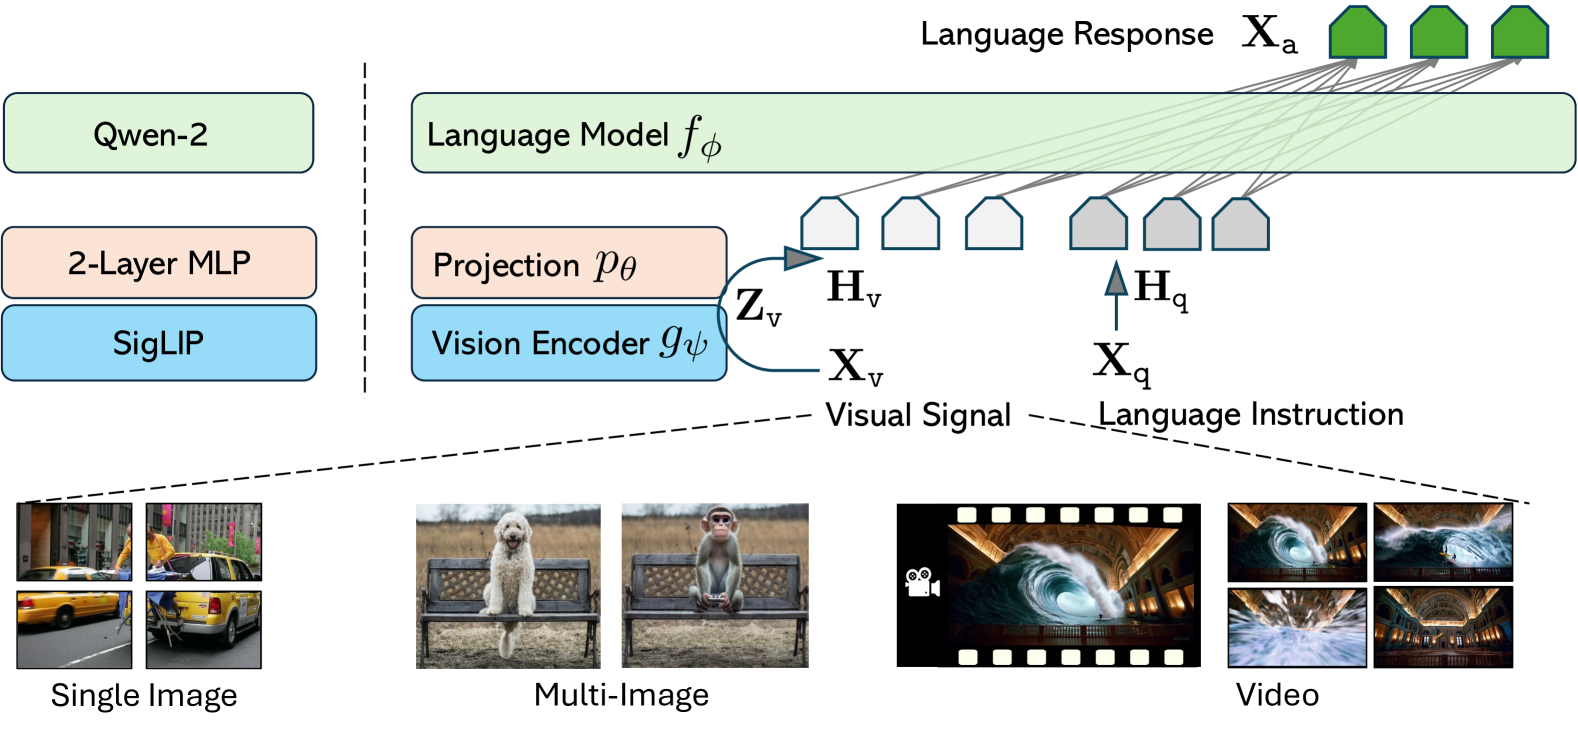
\includegraphics[width=\linewidth, height=0.58\textheight, keepaspectratio]{images/multimodal-nlp/multimodal_llava_onevision_architecture.png}
        \caption*{\scriptsize The recipe in 2024: SigLIP encoder, MLP projector, Qwen-2 LLM. Source: Li et al.,
        ``LLaVA-OneVision'', \href{https://arxiv.org/abs/2408.03326}{arXiv:2408.03326}, Figure~1.}
      \end{figure}
  \end{columns}
  \vspace{0.2em}
  {\scriptsize Liu et al., \href{https://arxiv.org/abs/2310.03744}{arXiv:2310.03744};
  Deitke et al., \href{https://arxiv.org/abs/2409.17146}{arXiv:2409.17146}.}
\end{frame}

\begin{frame}{How Images Become Tokens}
  \begin{columns}[T,onlytextwidth]
    \column{0.52\textwidth}
      \begin{itemize}
        \item[{\color{red}\textbullet}] \textbf{Patches are the atoms:} a ViT cuts the image into
          fixed-size patches. ViT-L/14 at $336\times336$ yields $(336/14)^2 = 576$ patch embeddings,
          the per-image token count of LLaVA-1.5.
        \item[{\color{red}\textbullet}] \textbf{Compression is a design axis:} BLIP-2's Q-Former distills
          every image into 32 learned query tokens; Flamingo's Perceiver Resampler emits 64.
        \item[{\color{red}\textbullet}] \textbf{Resolution multiplies cost:} AnyRes encodes each 336px
          tile separately; Qwen's native dynamic resolution merges each $2\times2$ patch group and spends
          tokens in proportion to image area.
        \item[{\color{red}\textbullet}] The trade-off between visual fidelity and context budget shapes
          every design in this lecture.
      \end{itemize}
    \column{0.44\textwidth}
      \begin{figure}
        \centering
        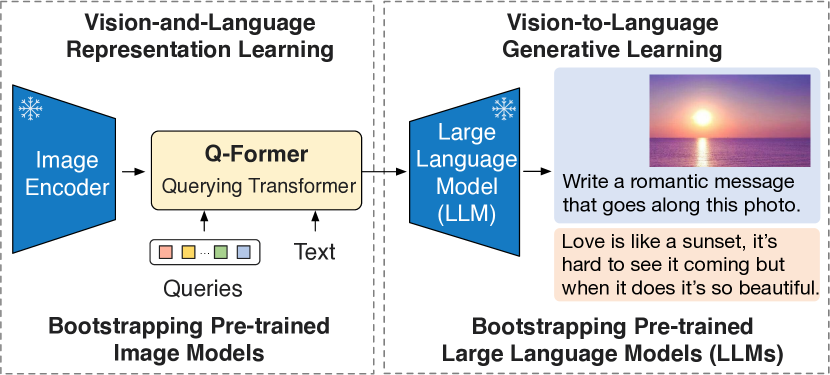
\includegraphics[width=\linewidth, height=0.52\textheight, keepaspectratio]{images/multimodal-nlp/multimodal_blip2_qformer_query_tokens.png}
        \caption*{\scriptsize BLIP-2's Q-Former: 32 learned queries distill a frozen encoder's features
        for a frozen LLM. Source: Li et al., BLIP-2, ICML 2023,
        \href{https://arxiv.org/abs/2301.12597}{arXiv:2301.12597}, Figure~1.}
      \end{figure}
  \end{columns}
\end{frame}
